% fig interference
\begin{figure}
% pgsplots code begins
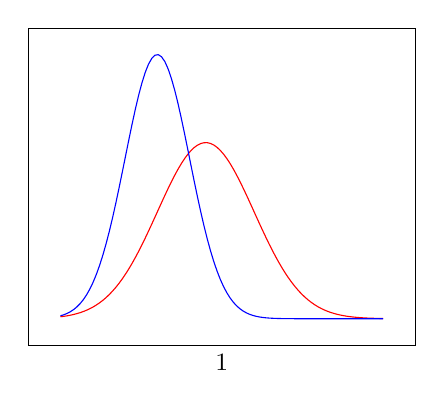
\begin{tikzpicture}[baseline] % baseline per pgsplots man
	\pgfmathdeclarefunction{gauss}{2}{\pgfmathparse{1/(#2*sqrt(2*pi))*exp(-((x-#1)^2)/(2*#2^2))}} % to use in \addplot
	\begin{axis}[
		small,
		xlabel=1, ylabel=, % labels
		xtick=\empty, ytick=\empty, % ticks
		]
	\addplot [
      red,
		domain=0:10,
		samples=100,
      ] {gauss(4.5, 1.5)};
	\addplot [
      blue,
      domain=0:10,
      samples=100,
      ] {gauss(3, 1)};
	\end{axis}
\end{tikzpicture}% \% here to avoid whitespace
\hskip 10pt % per pgsplot man
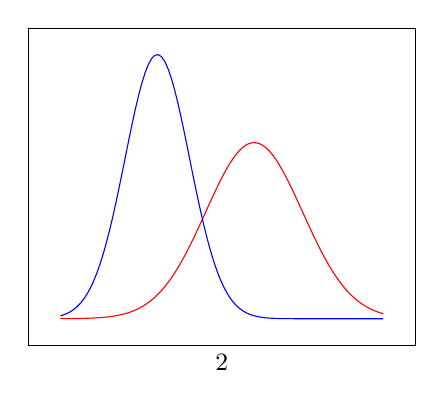
\begin{tikzpicture}[baseline] % baseline per pgsplots man
	\pgfmathdeclarefunction{gauss}{2}{\pgfmathparse{1/(#2*sqrt(2*pi))*exp(-((x-#1)^2)/(2*#2^2))}} % to use in \addplot
	\begin{axis}[
		small,
		yticklabel pos=upper,
		xlabel=2, ylabel=, % labels
		xtick=\empty, ytick=\empty, % ticks
		]
	\addplot [
      red,
		domain=0:10,
		samples=100,
		] {gauss(6, 1.5)};
	\addplot [
      blue,
      domain=0:10,
      samples=100,
      ] {gauss(3, 1)};
	\end{axis}
\end{tikzpicture}
% pgsplots code ends
\caption{Constructive vs destructive interference/close vs loose tracking/positive vs negative coincidence of piracy-yay* (blue) and piracy-nay* (red).}
\label{fig:yaynayinterference}
\end{figure}
%
